%% Part of Stellarium User Guide
%% Status: 2015-12-30 Some parts collected from wiki.
%%         2016-04-05 GZ changed to have 1 chapter per plugin for a better structure. This file may be split up later. 
%% TODO: All plugins! And give a better structure than just by alphabet.

\chapter{Angle Measure Plugin}
\label{sec:plugins:AngleMeasure}

%\url{http://porpoisehead.net/images/plugin-angle-measure.jpg}

The Angle Measure plugin is a small tool which is used to measure the
angular distance between two points on the sky. 

\small{*goes misty eyed*\\ 
I recall measuring the size of the Cassini Division when I was a student.
It was not the high academic glamor one might expect... It was cloudy...
It was rainy... The observatory lab had some old scopes set up at one
end, pointing at a \emph{photograph} of Saturn at the other end of the
lab. We measured. We calculated. We wished we were in Hawaii. A picture
is worth a thousand words.}

\section{Using the plugin}
\label{sec:plugins:AngleMeasure:using}

\begin{enumerate}
\item
  Enable the tool by clicking the tool-bar button, or by pressing
  \textbf{control-A}. A message will appear at the bottom of the screen
  to tell you that the tool is active.
\item
  Drag a line from the first point to the second point using the left
  mouse button
\item
  To clear the measurement, click the right mouse button
\item
  To deactivate the angle measure tool, press the tool-bar button again,
  or press \textbf{control-A} on the keyboard.
\end{enumerate}


\chapter{Bright Novae Plugin}
\label{sec:plugins:BrightNovae}

The Bright Novae plugin provides visualization of some bright novae in
the Milky Way galaxy (Fig.~\ref{fig:NovaCygni1975}).

%Example (\href{http://en.wikipedia.org/wiki/V1500_Cygni}{\textbf{Nova
%Cygni 1975}}, also known as \textbf{V1500 Cyg}):

\begin{figure}[h]
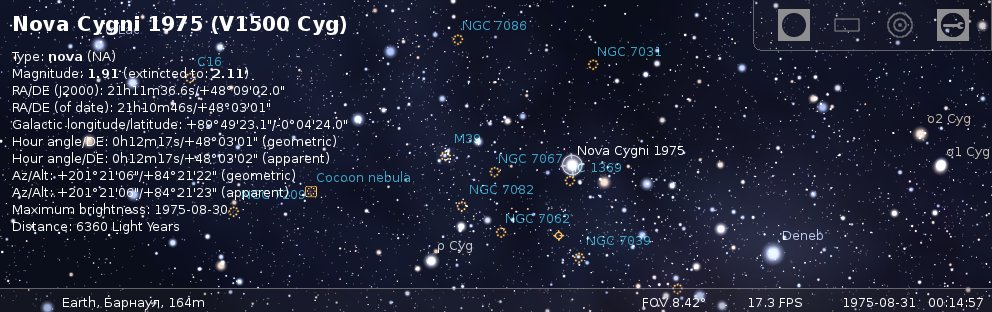
\includegraphics[width=\textwidth]{NovaCygni1975wiki.jpg}
\label{fig:NovaCygni1975}
\caption{Nova Cygni 1975 (also known as \textbf{V1500 Cyg})}
\end{figure}

\section{Using the Bright Novae plugin}
\label{sec:plugins:BrighrNovae:using}

\begin{enumerate}
\item Enable the tool by clicking the tool-bar button ``Load at startup''
\item Set date and time (30 August 1975 year for \emph{Nova Cygni 1975} as example\footnote{\url{http://en.wikipedia.org/wiki/V1500_Cygni}})
\end{enumerate}

\section{Section \big[Novae\big] in config.ini file}
\label{sec:plugins:BrightNovae:config}

You can edit \file{config.ini} file by yourself for changes of the
settings for the Bright Novae plugin -- just make it carefully!

\begin{longtabu} to \textwidth {l|l|X}\toprule
\emph{ID}            & \emph{Type} & \emph{Description}\\\midrule
last\_update            & string & Date and time of last update\\\midrule
update\_frequency\_days & int    & Frequency of updates, in days\\\midrule
updates\_enable         & bool   & Enable updates of bright novae catalog from Internet \\\midrule
url                     & string & URL of bright novae catalog \\\bottomrule
\end{longtabu}

\section{Format of bright novae catalog}
\label{sec:plugins:BrightNovae:format}

To add a new nova, open a new line after line 5 and paste the following, note commas and brackets, they are important:

\begin{configfile}
"Nova designation":
{
    "name": "name of nova",
    "type": "type of nova",
    "maxMagnitude": value of maximal visual magnitude,
    "minMagnitude": value of minimal visual magnitude,
    "peakJD": JD for maximal visual magnitude,
    "m2": Time to decline by 2mag from maximum (in days),
    "m3": Time to decline by 3mag from maximum (in days),
    "m6": Time to decline by 6mag from maximum (in days),
    "m9": Time to decline by 9mag from maximum (in days),
    "distance": value of distance between nova and 
                Earth (in thousands of Light Years),
    "RA": "Right ascension (J2000)",
    "Dec": "Declination (J2000)"
},
\end{configfile}

\newpage
\noindent For example, the record for \textbf{Nova Cygni 1975} (\textbf{V1500 Cyg}) looks like:
\begin{configfile}
"V1500 Cyg":
{
    "name": "Nova Cygni 1975",
    "type": "NA",
    "maxMagnitude": 1.69,
    "minMagnitude": 21,
    "peakJD": 2442655,
    "m2": 2,
    "m3": 4,
    "m6": 32,
    "m9": 263
    "distance": 6.36,
    "RA": "21h11m36.6s",
    "Dec": "48d09m02s"
},
\end{configfile}

\section{Light curves}
\label{sec:plugins:BrightNovae:lightcurves}

This plugin uses a very simple model for calculation of light curves for
novae stars. This model is based on time for decay by $N$
magnitudes from the maximum value, where $N$ is 2, 3, 6 and 9. If a
nova has no values for decay of magnitude then this plugin will use
generalized values for it.

\chapter{Compass Marks Plugin}
\label{sec:plugins:CompassMarks}

%\url{http://porpoisehead.net/images/plugin-compass-marks.jpg}

Stellarium helps the user get their bearings using the cardinal point
feature - the North, South, East and West markers on the horizon.
Compass Marks takes this idea and extends it to add markings every few
degrees along the horizon, and includes compass bearing values in
degrees.

\section{Using the plugin}
\label{sec:plugins:CompassMarks:using}

There is a tool bar button for toggling the compass markings, or you can
press \key{control-C}.

Note that when you first enable compass marks, the cardinal points will
be turned off. You can have both active at once, but there is a small
bug which means you have to press \key{Q} \emph{two times} to
re-enable cardinal points after enabling the compass markings.

\chapter{Pulsars Plugin}
\label{sec:plugins:Pulsars}

This plugin plots the position of various pulsars, with object information about each one. Pulsar data is derived from \textit{The ATNF Pulsar Catalogue} (Manchester, R. N., Hobbs, G. B., Teoh, A. \& Hobbs, M., Astron. J., 129, 1993-2006 (2005) (\href{http://arxiv.org/abs/astro-ph/0412641}{astro-ph/0412641})).

\begin{figure}[h]
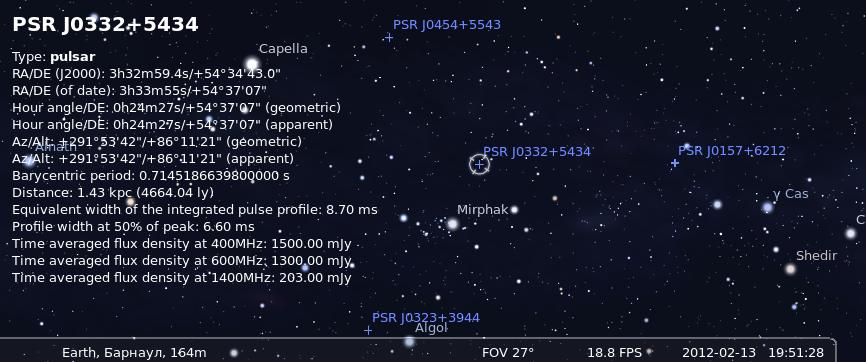
\includegraphics[width=\textwidth]{psr_j0332_5434.jpg}
\label{fig:PSR_J0332-5434}
\caption{PSR J0332-5434}
\end{figure}

\section{Using the Pulsars plugin}
\label{sec:plugins:Pulsars:using}

\begin{enumerate}
\item Enable the tool by clicking the tool-bar button ``Load at startup''
\item Find the pulsar by their designation (\emph{PSR J0437-4715} as example)
\end{enumerate}

\section{Section \big[Pulsars\big] in config.ini file}
\label{sec:plugins:Pulsars:config}

\begin{longtabu} to \textwidth {l|l|X}\toprule
\emph{ID}               & \emph{Type} & \emph{Description}\\\midrule
last\_update                & string & Date and time of last update\\\midrule
update\_frequency\_days     & int    & Frequency of updates, in days\\\midrule
updates\_enable             & bool   & Enable updates of pulsars catalog from Internet \\\midrule
url                         & string & URL of pulsars catalog \\\midrule
enable\_at\_startup         & bool   & Enable displaying of pulsars at startup of Stellarium \\\midrule
distribution\_enabled       & bool   & Enable distribution mode for the pulsars \\\midrule
flag\_show\_pulsars\_button & bool   & Enable displaying pulsars button on toolbar \\\midrule
marker\_color               & R,G,B  & Color for marker of the pulsars \\\midrule
glitch\_color               & R,G,B  & Color for marker of the pulsars with glitches \\\midrule
use\_separate\_colors       & bool   & Use separate colors for different types of the pulsars \\\bottomrule
\end{longtabu}

\section{Format of pulsars catalog}
\label{sec:plugins:Pulsars:format}

To add a new pulsar, open a new line after line 5 and paste the following, note commas and brackets, they are important:

%\newpage

\begin{configfile}
"Pulsar designation":
{
    "RA": "Right ascension (J2000)",
    "DE": "Declination (J2000)",
    "notes": "type of pulsar",
    "distance": value of distance based on electron density 
                model (kpc),
    "period": value of barycentric period of the pulsar (s),
    "parallax": value of annular parallax (mas),
    "bperiod": value of binary period of pulsar (days),
    "pderivative": value of time derivative of barcycentric 
                   period,
    "dmeasure": value of dispersion measure (cm^-3 pc),
    "frequency": value of barycentric rotation frequency (Hz),
    "pfrequency": value of time derivative of barycentric 
                  rotation frequency (s^-2)
    "eccentricity": value of eccentricity,                   
    "w50": value of profile width at 50% of peak (ms),
    "s400": value of time averaged flux density at 
            400 MHz (mJy),
    "s600": value of time averaged flux density at 
            600 MHz (mJy),
    "s1400": value of time averaged flux density at 
             1400 MHz (mJy)    
},

\end{configfile}

%\newpage
\noindent For example, the record for \textbf{PSR J0014+4746} looks like:
\begin{configfile}
"PSR J0014+4746":
{
    "distance": 1.82,
    "dmeasure": 30.85,
    "frequency": 0.805997239145,
    "pfrequency": -3.6669E-16,
    "w50": 88.7,
    "s400": 14,
    "s600": 9,
    "s1400": 3,
    "RA": "00h14m17.75s",
    "DE": "47d46m33.4s"
},
\end{configfile}



\chapter{Text User Interface}
\label{sec:plugins:TextUserInterface}

%\url{http://porpoisehead.net/images/plugin-tui.jpg}

Older versions of Stellarium used to have a little menu system which was
controlled by the cursor keys. This was used primarily by planetarium
system operators to change settings, run scripts and so on. In the
0.10.x series, this function vanished as we totally re-designed the user
interface. This plugin re-implements the ``TUI'', as it was known. Full
list of the commands for the TUI plugin you can read in the section
\href{TUI_Commands}{TUI Commands}.

\section{Using the Text User Interface}
\label{sec:plugins:TUI:using}

\begin{enumerate}
\item Activate the text menu using the \key{Alt-T} key.\footnote{This
    used to be hard-coded to \key{M} before version 0.15, but
    \key{Alt-T} runs parallel with \key{Ctrl-T} for switching the GUI
    panels, and frees up \key{M} for the Milky Way. The \key{Alt-T}
    keybinding is hardcoded, i.e., cannot be reconfigured by the
    user.}
\item
  Navigate the menu using the cursors keys.
\item
  To edit a value, press the right cursor until the value you wish to
  change it highlighted with \textgreater{} and \textless{} marks, e.g.\
  \textgreater{}3.142\textless{}. Then press the up and down cursors to
  change the value. You may also type in a new value with the other keys
  on the keyboard.
\end{enumerate}

\section{TUI Commands}
\label{sec:plugins:TUI:commands}
\begin{longtabu} to \textwidth {l|l|X}
\toprule
1   & Set Location & (menu group)\\\midrule
1.1 & Latitude & Set the latitude of the observer in degrees\\\midrule
1.2 & Longitude & Set the longitude of the observer in degrees\\\midrule
1.3 & Altitude (m) & Set the altitude of the observer in meters\\\midrule
1.4 & Solar System Body & Select the solar system body on which the observer is\\\midrule
2   & Set Time & (menu group)\\\midrule
2.1 & Sky Time & Set the time and date for which Stellarium will generate the view\\\midrule
2.2 & Set Time Zone & Set the time zone. Zones are split into continent or region, and then by city or province\\\midrule
2.3 & Days keys & The setting ``Calendar'' makes the - = {[} {]} and keys change the date value by calendar days (multiples of 24 hours). 
                  The setting ``Sidereal day'' changes these keys to change the date by sidereal days\\\midrule
2.4 & Preset Sky Time & Select the time which Stellarium starts with (if the ``Sky Time At Start-up'' setting is ``Preset Time''\\\midrule
2.5 & Sky Time At Start-up & The setting ``Actual Time'' sets Stellarium's time to the computer clock when Stellarium runs. 
                             The setting ``Preset Time'' selects a time set in menu item ``Preset Sky Time''\\\midrule
2.6 & Time Display Format & Change how Stellarium formats time values. ``system default'' takes the format from the computer settings, 
                            or it is possible to select 24 hour or 12 hour clock modes\\\midrule
2.7 & Date Display Format & Change how Stellarium formats date values. ``system default'' takes the format from the computer settings, 
                            or it is possible to select ``yyyymmdd'', ``ddmmyyyy'' or ``mmddyyyy'' modes\\\midrule
3    & General & (menu group)\\\midrule
3.1  & Sky Culture  & Select the sky culture to use (changes constellation lines, names, artwork)\\\midrule
3.2  & Sky Language & Change the language used to describe objects in the sky\\\midrule
4    & Stars & (menu group)\\\midrule
4.1  & Show & Turn on/off star rendering\\\midrule
4.2  & Star Magnitude Multiplier & Can be used to change the brightness of the stars which are visible at a given zoom level. 
                                   This may be used to simulate local seeing conditions - the lower the value, the less stars will be visible\\\midrule
4.3  & Maximum Magnitude to Label & Changes how many stars get labelled according to their apparent magnitude (if star labels are turned on)\\\midrule
4.4  & Twinkling & Sets how strong the star twinkling effect is - zero is off, the higher the value the more the stars will twinkle.\\\midrule
5    & Colors & (menu group)\\\midrule
5.1  & Constellation Lines         & Changes the colour of the constellation lines\\\midrule
5.2  & Constellation Names         & Changes the colour of the labels used to name stars\\\midrule
5.3  & Constellation Art Intensity & Changes the brightness of the constellation artconstellation art\\\midrule
5.4  & Constellation Boundaries    & Changes the colour of the constellation boundary lines\\\midrule
5.5  & Cardinal Points & Changes the colour of the cardinal points markers\\\midrule
5.6  & Planet Names    & Changes the colour of the labels for planets\\\midrule
5.7  & Planet Orbits   & Changes the colour of the orbital guide lines for planets\\\midrule
5.8  & Planet Trails   & Changes the colour of the planet trails lines\\\midrule
5.9  & Meridian Line   & Changes the colour of the meridian line\\\midrule
5.10 & Azimuthal Grid  & Changes the colour of the lines and labels for the azimuthal grid\\\midrule
5.11 & Equatorial Grid & Changes the colour of the lines and labels for the equatorial grid\\\midrule
5.12 & Equator Line    & Changes the colour of the equator line\\\midrule
5.13 & Ecliptic Line   & Changes the colour of the ecliptic line\\\midrule
5.14 & Nebula Names    & Changes the colour of the labels for nebulae\\\midrule
5.15 & Nebula Circles  & Changes the colour of the circles used to denote the positions of nebulae (only when enabled int he configuration file, note this feature is off by default)\\\midrule
6   & Effects & (menu group)\\\midrule
6.1 & Light Pollution Luminance & Changes the intensity of the light pollution simulation\\\midrule
6.2 & Landscape & Used to select the landscape which Stellarium draws when ground drawing is enabled\\\midrule
6.3 & Manual zoom & Changes the behaviour of the \key{/} and \key{\textbackslash{}} keys. When set to ``No'', these keys zoom all the way to a level defined
by object type (auto zoom mode). When set to ``Yes'', these keys zoom in and out a smaller amount and multiple presses are required\\\midrule
6.4 & Object Sizing Rule & When set to ``Magnitude'', stars are drawn with a size based on their apparent magnitude. When set to ``Point'' all stars are drawn with the same size on the screen\\\midrule
6.5 & Magnitude Sizing Multiplier & Changes the size of the stars when ``Object Sizing Rule'' is set to ``Magnitude''\\\midrule
6.6 & Milky Way intensity & Changes the brightness of the Milky Way texture\\\midrule
6.7 & Maximum Nebula Magnitude to Label & Changes the magnitude limit for labelling of nebulae\\\midrule
6.8 & Zoom Duration & Sets the time for zoom operations to take (in seconds)\\\midrule
6.9 & Cursor Timeout & Sets the number of seconds of mouse inactivity before the cursor vanishes\\\midrule
6.10 & Setting Landscape Sets Location & If ``Yes'' then changing the landscape will move the observer location to the location for that landscape (if one is known). 
                                         Setting this to ``No'' means the observer location is not modified when the landscape is changed.\\\midrule
7 & Scripts & (menu group)\\\midrule
7.1 & Local Script & Run a script from the scripts sub-directory of the User Directory or Installation Directory (see section~\ref{sec:FilesAndDirectories} (Files and Directories))\\\midrule
7.2 & CD/DVD Script          & Run a script from a CD or DVD (only used in planetarium set-ups)\\\midrule
8   & Administration         & (menu group)\\\midrule
8.1 & Load Default Configuration & Reset all settings according to the main configuration file\\\midrule
8.2 & Save Current Configuration as Default & Save the current settings to the main configuration file\\\midrule
8.3 & Shutdown               & Quit Stellarium\\\midrule
8.4 & Update me via Internet & Only used in planetarium set-ups\\\midrule
8.5 & Set UI Locale          & Change the language used for the user interface\\\bottomrule
\end{longtabu}




%%% Local Variables: 
%%% mode: latex
%%% TeX-master: "guide"
%%% End: 

